\tikzset{every picture/.style={line width=0.75pt}} %set default line width to 0.75pt        

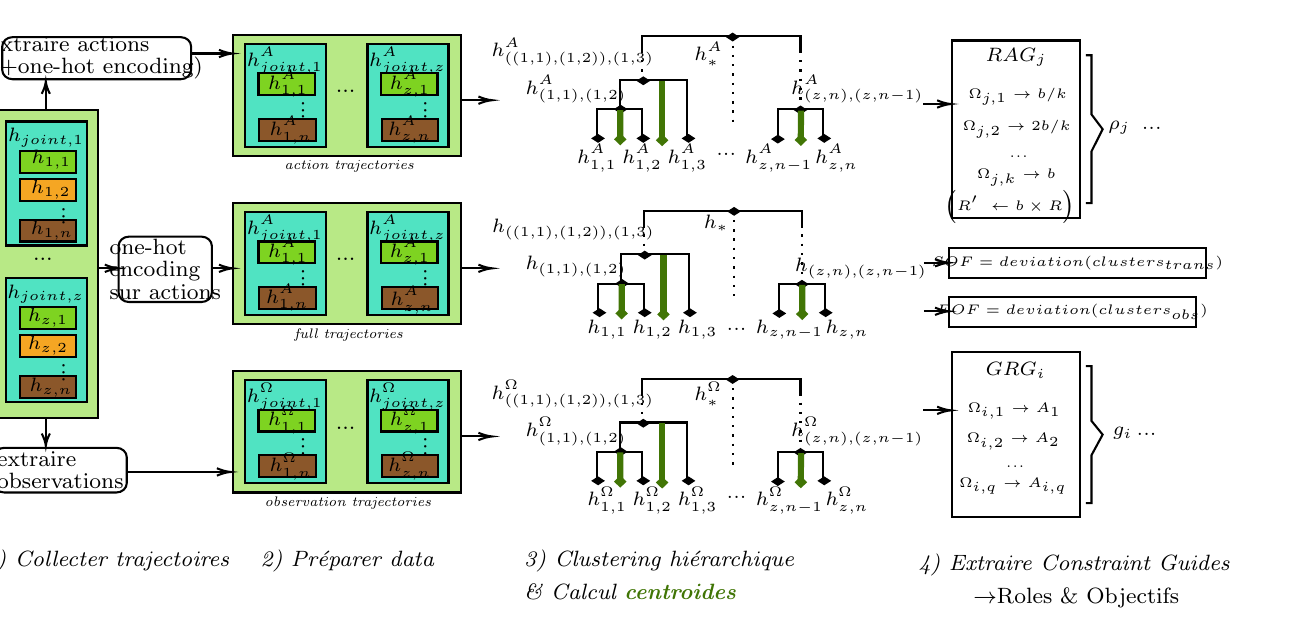
\begin{tikzpicture}[x=0.75pt,y=0.75pt,yscale=-0.9,xscale=1]
%uncomment if require: \path (0,1723); %set diagram left start at 0, and has height of 1723

\hspace{-0.6cm}

%Shape: Rectangle [id:dp09610487374035748] 
\draw  [fill={rgb, 255:red, 184; green, 233; blue, 134 }  ,fill opacity=1 ] (30,1232) -- (80,1232) -- (80,1397) -- (30,1397) -- cycle ;
%Shape: Rectangle [id:dp45316125392913] 
\draw  [fill={rgb, 255:red, 80; green, 227; blue, 194 }  ,fill opacity=1 ] (35.96,1238.4) -- (74.96,1238.4) -- (74.96,1304.76) -- (35.96,1304.76) -- cycle ;
%Shape: Rectangle [id:dp45830823192172254] 
\draw  [fill={rgb, 255:red, 245; green, 166; blue, 35 }  ,fill opacity=1 ] (42.44,1269.04) -- (69.69,1269.04) -- (69.69,1280.75) -- (42.44,1280.75) -- cycle ;
%Shape: Rectangle [id:dp3946596851341897] 
\draw  [fill={rgb, 255:red, 139; green, 87; blue, 42 }  ,fill opacity=1 ] (42.44,1290.91) -- (69.69,1290.91) -- (69.69,1302.62) -- (42.44,1302.62) -- cycle ;
%Shape: Rectangle [id:dp12555529945477895] 
\draw  [fill={rgb, 255:red, 126; green, 211; blue, 33 }  ,fill opacity=1 ] (42.44,1254.01) -- (69.69,1254.01) -- (69.69,1265.72) -- (42.44,1265.72) -- cycle ;
%Shape: Rectangle [id:dp7349415985100746] 
\draw  [fill={rgb, 255:red, 80; green, 227; blue, 194 }  ,fill opacity=1 ] (36,1322) -- (75,1322) -- (75,1388.37) -- (36,1388.37) -- cycle ;
%Shape: Rectangle [id:dp26642582947795324] 
\draw  [fill={rgb, 255:red, 245; green, 166; blue, 35 }  ,fill opacity=1 ] (42.48,1352.65) -- (69.72,1352.65) -- (69.72,1364.36) -- (42.48,1364.36) -- cycle ;
%Shape: Rectangle [id:dp9632684060086679] 
\draw  [fill={rgb, 255:red, 139; green, 87; blue, 42 }  ,fill opacity=1 ] (42.48,1374.51) -- (69.72,1374.51) -- (69.72,1386.22) -- (42.48,1386.22) -- cycle ;
%Shape: Rectangle [id:dp0008867618580383763] 
\draw  [fill={rgb, 255:red, 126; green, 211; blue, 33 }  ,fill opacity=1 ] (42.48,1337.62) -- (69.72,1337.62) -- (69.72,1349.33) -- (42.48,1349.33) -- cycle ;
%Shape: Rectangle [id:dp5049511033223727] 
\draw  [fill={rgb, 255:red, 255; green, 255; blue, 255 }  ,fill opacity=1 ] (30,1418.08) .. controls (30,1415.32) and (32.24,1413.08) .. (35,1413.08) -- (89,1413.08) .. controls (91.76,1413.08) and (94,1415.32) .. (94,1418.08) -- (94,1432) .. controls (94,1434.76) and (91.76,1437) .. (89,1437) -- (35,1437) .. controls (32.24,1437) and (30,1434.76) .. (30,1432) -- cycle ;

%Shape: Rectangle [id:dp861803318395177] 
\draw  [fill={rgb, 255:red, 184; green, 233; blue, 134 }  ,fill opacity=1 ] (145,1192) -- (255,1192) -- (255,1257) -- (145,1257) -- cycle ;
%Shape: Rectangle [id:dp6132217248920296] 
\draw  [fill={rgb, 255:red, 80; green, 227; blue, 194 }  ,fill opacity=1 ] (151,1197) -- (190,1197) -- (190,1252) -- (151,1252) -- cycle ;
%Shape: Rectangle [id:dp5733108309348334] 
\draw  [fill={rgb, 255:red, 139; green, 87; blue, 42 }  ,fill opacity=1 ] (157.76,1237) -- (185,1237) -- (185,1248.71) -- (157.76,1248.71) -- cycle ;
%Shape: Rectangle [id:dp2842929693852999] 
\draw  [fill={rgb, 255:red, 126; green, 211; blue, 33 }  ,fill opacity=1 ] (157.48,1212.62) -- (184.72,1212.62) -- (184.72,1224.33) -- (157.48,1224.33) -- cycle ;
%Shape: Rectangle [id:dp56024471923465] 
\draw  [fill={rgb, 255:red, 80; green, 227; blue, 194 }  ,fill opacity=1 ] (210,1197) -- (249,1197) -- (249,1252) -- (210,1252) -- cycle ;
%Shape: Rectangle [id:dp762658002129142] 
\draw  [fill={rgb, 255:red, 139; green, 87; blue, 42 }  ,fill opacity=1 ] (216.76,1237) -- (244,1237) -- (244,1248.71) -- (216.76,1248.71) -- cycle ;
%Shape: Rectangle [id:dp17126433901717386] 
\draw  [fill={rgb, 255:red, 126; green, 211; blue, 33 }  ,fill opacity=1 ] (216.48,1212.62) -- (243.72,1212.62) -- (243.72,1224.33) -- (216.48,1224.33) -- cycle ;
%Shape: Rectangle [id:dp9537774458308554] 
\draw  [fill={rgb, 255:red, 184; green, 233; blue, 134 }  ,fill opacity=1 ] (145,1372) -- (255,1372) -- (255,1437) -- (145,1437) -- cycle ;
%Shape: Rectangle [id:dp7233105184708959] 
\draw  [fill={rgb, 255:red, 80; green, 227; blue, 194 }  ,fill opacity=1 ] (151,1377) -- (190,1377) -- (190,1432) -- (151,1432) -- cycle ;
%Shape: Rectangle [id:dp6105572959886556] 
\draw  [fill={rgb, 255:red, 139; green, 87; blue, 42 }  ,fill opacity=1 ] (157.76,1417) -- (185,1417) -- (185,1428.71) -- (157.76,1428.71) -- cycle ;
%Shape: Rectangle [id:dp12021735107027742] 
\draw  [fill={rgb, 255:red, 126; green, 211; blue, 33 }  ,fill opacity=1 ] (157.48,1392.62) -- (184.72,1392.62) -- (184.72,1404.33) -- (157.48,1404.33) -- cycle ;
%Shape: Rectangle [id:dp013850868214046685] 
\draw  [fill={rgb, 255:red, 80; green, 227; blue, 194 }  ,fill opacity=1 ] (210,1377) -- (249,1377) -- (249,1432) -- (210,1432) -- cycle ;
%Shape: Rectangle [id:dp18055620205595135] 
\draw  [fill={rgb, 255:red, 139; green, 87; blue, 42 }  ,fill opacity=1 ] (216.76,1417) -- (244,1417) -- (244,1428.71) -- (216.76,1428.71) -- cycle ;
%Shape: Rectangle [id:dp8438669395198585] 
\draw  [fill={rgb, 255:red, 126; green, 211; blue, 33 }  ,fill opacity=1 ] (216.48,1392.62) -- (243.72,1392.62) -- (243.72,1404.33) -- (216.48,1404.33) -- cycle ;
%Straight Lines [id:da3008118547681833] 
\draw    (125,1202) -- (143,1202) ;
\draw [shift={(145,1202)}, rotate = 180] [color={rgb, 255:red, 0; green, 0; blue, 0 }  ][line width=0.75]    (6.56,-1.97) .. controls (4.17,-0.84) and (1.99,-0.18) .. (0,0) .. controls (1.99,0.18) and (4.17,0.84) .. (6.56,1.97)   ;
%Shape: Rectangle [id:dp31005292076420676] 
\draw  [fill={rgb, 255:red, 255; green, 255; blue, 255 }  ,fill opacity=1 ] (34,1198.24) .. controls (34,1195.48) and (36.24,1193.24) .. (39,1193.24) -- (120,1193.24) .. controls (122.76,1193.24) and (125,1195.48) .. (125,1198.24) -- (125,1210.76) .. controls (125,1213.52) and (122.76,1215.76) .. (120,1215.76) -- (39,1215.76) .. controls (36.24,1215.76) and (34,1213.52) .. (34,1210.76) -- cycle ;

%Straight Lines [id:da867093953960449] 
\draw    (55,1232) -- (55,1219) ;
\draw [shift={(55,1217)}, rotate = 90] [color={rgb, 255:red, 0; green, 0; blue, 0 }  ][line width=0.75]    (6.56,-1.97) .. controls (4.17,-0.84) and (1.99,-0.18) .. (0,0) .. controls (1.99,0.18) and (4.17,0.84) .. (6.56,1.97)   ;
%Straight Lines [id:da09509111300082773] 
\draw    (55,1397) -- (55,1410) ;
\draw [shift={(55,1412)}, rotate = 270] [color={rgb, 255:red, 0; green, 0; blue, 0 }  ][line width=0.75]    (6.56,-1.97) .. controls (4.17,-0.84) and (1.99,-0.18) .. (0,0) .. controls (1.99,0.18) and (4.17,0.84) .. (6.56,1.97)   ;
%Straight Lines [id:da37053818789319803] 
\draw    (320.53,1430.76) -- (320.53,1415.15) -- (342.33,1415.15) -- (342.33,1430.76) ;
%Straight Lines [id:da27331471605364943] 
\draw    (331.43,1415.15) -- (331.43,1399.53) -- (364.12,1399.53) -- (364.12,1430.76) ;
%Straight Lines [id:da4312567064966427] 
\draw    (342.33,1383.91) -- (342.33,1376.11) -- (418.61,1376.11) -- (418.61,1383.91) ;
%Straight Lines [id:da22888172465679524] 
\draw    (407.71,1430.76) -- (407.71,1415.15) -- (429.51,1415.15) -- (429.51,1430.76) ;
%Shape: Ellipse [id:dp6184217681327564] 
\draw  [line width=2.25]  (320.53,1430.76) .. controls (320.53,1430.55) and (320.78,1430.37) .. (321.08,1430.37) .. controls (321.38,1430.37) and (321.62,1430.55) .. (321.62,1430.76) .. controls (321.62,1430.98) and (321.38,1431.15) .. (321.08,1431.15) .. controls (320.78,1431.15) and (320.53,1430.98) .. (320.53,1430.76) -- cycle ;
%Shape: Ellipse [id:dp06577345173315474] 
\draw  [line width=2.25]  (342.33,1430.76) .. controls (342.33,1430.55) and (342.57,1430.37) .. (342.87,1430.37) .. controls (343.17,1430.37) and (343.42,1430.55) .. (343.42,1430.76) .. controls (343.42,1430.98) and (343.17,1431.15) .. (342.87,1431.15) .. controls (342.57,1431.15) and (342.33,1430.98) .. (342.33,1430.76) -- cycle ;
%Shape: Ellipse [id:dp7107422628707226] 
\draw  [line width=2.25]  (364.12,1430.76) .. controls (364.12,1430.55) and (364.37,1430.37) .. (364.67,1430.37) .. controls (364.97,1430.37) and (365.21,1430.55) .. (365.21,1430.76) .. controls (365.21,1430.98) and (364.97,1431.15) .. (364.67,1431.15) .. controls (364.37,1431.15) and (364.12,1430.98) .. (364.12,1430.76) -- cycle ;
%Shape: Ellipse [id:dp6939382648562396] 
\draw  [line width=2.25]  (407.17,1431.15) .. controls (407.17,1430.94) and (407.41,1430.76) .. (407.71,1430.76) .. controls (408.01,1430.76) and (408.26,1430.94) .. (408.26,1431.15) .. controls (408.26,1431.37) and (408.01,1431.54) .. (407.71,1431.54) .. controls (407.41,1431.54) and (407.17,1431.37) .. (407.17,1431.15) -- cycle ;
%Shape: Ellipse [id:dp08118677913158812] 
\draw  [line width=2.25]  (429.51,1430.76) .. controls (429.51,1430.55) and (429.75,1430.37) .. (430.05,1430.37) .. controls (430.35,1430.37) and (430.6,1430.55) .. (430.6,1430.76) .. controls (430.6,1430.98) and (430.35,1431.15) .. (430.05,1431.15) .. controls (429.75,1431.15) and (429.51,1430.98) .. (429.51,1430.76) -- cycle ;
%Shape: Ellipse [id:dp9493188068363742] 
\draw  [line width=2.25]  (331.43,1415.15) .. controls (331.43,1414.93) and (331.67,1414.75) .. (331.97,1414.75) .. controls (332.27,1414.75) and (332.52,1414.93) .. (332.52,1415.15) .. controls (332.52,1415.36) and (332.27,1415.54) .. (331.97,1415.54) .. controls (331.67,1415.54) and (331.43,1415.36) .. (331.43,1415.15) -- cycle ;
%Shape: Ellipse [id:dp31776400962313445] 
\draw  [line width=2.25]  (342.33,1399.92) .. controls (342.33,1399.7) and (342.57,1399.53) .. (342.87,1399.53) .. controls (343.17,1399.53) and (343.42,1399.7) .. (343.42,1399.92) .. controls (343.42,1400.14) and (343.17,1400.31) .. (342.87,1400.31) .. controls (342.57,1400.31) and (342.33,1400.14) .. (342.33,1399.92) -- cycle ;
%Shape: Ellipse [id:dp156886046038465] 
\draw  [line width=2.25]  (385.37,1376.5) .. controls (385.37,1376.28) and (385.62,1376.11) .. (385.92,1376.11) .. controls (386.22,1376.11) and (386.46,1376.28) .. (386.46,1376.5) .. controls (386.46,1376.71) and (386.22,1376.89) .. (385.92,1376.89) .. controls (385.62,1376.89) and (385.37,1376.71) .. (385.37,1376.5) -- cycle ;
%Shape: Ellipse [id:dp4090467774188007] 
\draw  [line width=2.25]  (418.06,1415.54) .. controls (418.06,1415.32) and (418.31,1415.15) .. (418.61,1415.15) .. controls (418.91,1415.15) and (419.15,1415.32) .. (419.15,1415.54) .. controls (419.15,1415.75) and (418.91,1415.93) .. (418.61,1415.93) .. controls (418.31,1415.93) and (418.06,1415.75) .. (418.06,1415.54) -- cycle ;
%Straight Lines [id:da5835970444465544] 
\draw  [dash pattern={on 0.84pt off 2.51pt}]  (342.33,1383.91) -- (342.33,1399.53) ;
%Straight Lines [id:da1689158486837592] 
\draw  [dash pattern={on 0.84pt off 2.51pt}]  (418.61,1383.91) -- (418.61,1415.15) ;
%Straight Lines [id:da2070689850273354] 
\draw  [dash pattern={on 0.84pt off 2.51pt}]  (385.92,1376.11) -- (385.92,1422.95) ;
%Straight Lines [id:da21678640379690228] 
\draw    (321.22,1340.76) -- (321.22,1325.15) -- (343.02,1325.15) -- (343.02,1340.76) ;
%Straight Lines [id:da3653267745057789] 
\draw    (332.12,1325.15) -- (332.12,1309.53) -- (364.81,1309.53) -- (364.81,1340.76) ;
%Straight Lines [id:da9487811381350612] 
\draw    (343.02,1293.91) -- (343.02,1286.11) -- (419.3,1286.11) -- (419.3,1293.91) ;
%Straight Lines [id:da6273772791005832] 
\draw    (408.4,1340.76) -- (408.4,1325.15) -- (430.2,1325.15) -- (430.2,1340.76) ;
%Shape: Ellipse [id:dp361908442745964] 
\draw  [line width=2.25]  (321.22,1340.76) .. controls (321.22,1340.55) and (321.47,1340.37) .. (321.77,1340.37) .. controls (322.07,1340.37) and (322.31,1340.55) .. (322.31,1340.76) .. controls (322.31,1340.98) and (322.07,1341.15) .. (321.77,1341.15) .. controls (321.47,1341.15) and (321.22,1340.98) .. (321.22,1340.76) -- cycle ;
%Shape: Ellipse [id:dp34035499911302736] 
\draw  [line width=2.25]  (343.02,1340.76) .. controls (343.02,1340.55) and (343.26,1340.37) .. (343.56,1340.37) .. controls (343.87,1340.37) and (344.11,1340.55) .. (344.11,1340.76) .. controls (344.11,1340.98) and (343.87,1341.15) .. (343.56,1341.15) .. controls (343.26,1341.15) and (343.02,1340.98) .. (343.02,1340.76) -- cycle ;
%Shape: Ellipse [id:dp8093356810114974] 
\draw  [line width=2.25]  (364.81,1340.76) .. controls (364.81,1340.55) and (365.06,1340.37) .. (365.36,1340.37) .. controls (365.66,1340.37) and (365.9,1340.55) .. (365.9,1340.76) .. controls (365.9,1340.98) and (365.66,1341.15) .. (365.36,1341.15) .. controls (365.06,1341.15) and (364.81,1340.98) .. (364.81,1340.76) -- cycle ;
%Shape: Ellipse [id:dp6886301228573949] 
\draw  [line width=2.25]  (407.86,1341.15) .. controls (407.86,1340.94) and (408.1,1340.76) .. (408.4,1340.76) .. controls (408.71,1340.76) and (408.95,1340.94) .. (408.95,1341.15) .. controls (408.95,1341.37) and (408.71,1341.54) .. (408.4,1341.54) .. controls (408.1,1341.54) and (407.86,1341.37) .. (407.86,1341.15) -- cycle ;
%Shape: Ellipse [id:dp6104880437237735] 
\draw  [line width=2.25]  (430.2,1340.76) .. controls (430.2,1340.55) and (430.44,1340.37) .. (430.74,1340.37) .. controls (431.05,1340.37) and (431.29,1340.55) .. (431.29,1340.76) .. controls (431.29,1340.98) and (431.05,1341.15) .. (430.74,1341.15) .. controls (430.44,1341.15) and (430.2,1340.98) .. (430.2,1340.76) -- cycle ;
%Shape: Ellipse [id:dp3847126134177271] 
\draw  [line width=2.25]  (332.12,1325.15) .. controls (332.12,1324.93) and (332.37,1324.75) .. (332.67,1324.75) .. controls (332.97,1324.75) and (333.21,1324.93) .. (333.21,1325.15) .. controls (333.21,1325.36) and (332.97,1325.54) .. (332.67,1325.54) .. controls (332.37,1325.54) and (332.12,1325.36) .. (332.12,1325.15) -- cycle ;
%Shape: Ellipse [id:dp9172247745940925] 
\draw  [line width=2.25]  (343.02,1309.92) .. controls (343.02,1309.7) and (343.26,1309.53) .. (343.56,1309.53) .. controls (343.87,1309.53) and (344.11,1309.7) .. (344.11,1309.92) .. controls (344.11,1310.14) and (343.87,1310.31) .. (343.56,1310.31) .. controls (343.26,1310.31) and (343.02,1310.14) .. (343.02,1309.92) -- cycle ;
%Shape: Ellipse [id:dp4031282586521814] 
\draw  [line width=2.25]  (386.06,1286.5) .. controls (386.06,1286.28) and (386.31,1286.11) .. (386.61,1286.11) .. controls (386.91,1286.11) and (387.15,1286.28) .. (387.15,1286.5) .. controls (387.15,1286.71) and (386.91,1286.89) .. (386.61,1286.89) .. controls (386.31,1286.89) and (386.06,1286.71) .. (386.06,1286.5) -- cycle ;
%Shape: Ellipse [id:dp010476775151872508] 
\draw  [line width=2.25]  (418.76,1325.54) .. controls (418.76,1325.32) and (419,1325.15) .. (419.3,1325.15) .. controls (419.6,1325.15) and (419.85,1325.32) .. (419.85,1325.54) .. controls (419.85,1325.75) and (419.6,1325.93) .. (419.3,1325.93) .. controls (419,1325.93) and (418.76,1325.75) .. (418.76,1325.54) -- cycle ;
%Straight Lines [id:da6762017945408133] 
\draw  [dash pattern={on 0.84pt off 2.51pt}]  (343.02,1293.91) -- (343.02,1309.53) ;
%Straight Lines [id:da9097085331303272] 
\draw  [dash pattern={on 0.84pt off 2.51pt}]  (419.3,1293.91) -- (419.3,1325.15) ;
%Straight Lines [id:da20995347959711252] 
\draw  [dash pattern={on 0.84pt off 2.51pt}]  (386.61,1286.11) -- (386.61,1332.95) ;
%Straight Lines [id:da300589271672265] 
\draw    (320.53,1247.44) -- (320.53,1231.82) -- (342.33,1231.82) -- (342.33,1247.44) ;
%Straight Lines [id:da7941749924863761] 
\draw    (331.43,1231.82) -- (331.43,1216.21) -- (364.12,1216.21) -- (364.12,1247.44) ;
%Straight Lines [id:da036984986996662195] 
\draw    (342.33,1200.59) -- (342.33,1192.78) -- (418.61,1192.78) -- (418.61,1200.59) ;
%Straight Lines [id:da2521545303562105] 
\draw    (407.71,1247.44) -- (407.71,1231.82) -- (429.51,1231.82) -- (429.51,1247.44) ;
%Shape: Ellipse [id:dp8674458972711949] 
\draw  [line width=2.25]  (320.53,1247.44) .. controls (320.53,1247.22) and (320.78,1247.05) .. (321.08,1247.05) .. controls (321.38,1247.05) and (321.62,1247.22) .. (321.62,1247.44) .. controls (321.62,1247.66) and (321.38,1247.83) .. (321.08,1247.83) .. controls (320.78,1247.83) and (320.53,1247.66) .. (320.53,1247.44) -- cycle ;
%Shape: Ellipse [id:dp40445696985977] 
\draw  [line width=2.25]  (342.33,1247.44) .. controls (342.33,1247.22) and (342.57,1247.05) .. (342.87,1247.05) .. controls (343.17,1247.05) and (343.42,1247.22) .. (343.42,1247.44) .. controls (343.42,1247.66) and (343.17,1247.83) .. (342.87,1247.83) .. controls (342.57,1247.83) and (342.33,1247.66) .. (342.33,1247.44) -- cycle ;
%Shape: Ellipse [id:dp9379775866500679] 
\draw  [line width=2.25]  (364.12,1247.44) .. controls (364.12,1247.22) and (364.37,1247.05) .. (364.67,1247.05) .. controls (364.97,1247.05) and (365.21,1247.22) .. (365.21,1247.44) .. controls (365.21,1247.66) and (364.97,1247.83) .. (364.67,1247.83) .. controls (364.37,1247.83) and (364.12,1247.66) .. (364.12,1247.44) -- cycle ;
%Shape: Ellipse [id:dp9822823316274046] 
\draw  [line width=2.25]  (407.17,1247.83) .. controls (407.17,1247.61) and (407.41,1247.44) .. (407.71,1247.44) .. controls (408.01,1247.44) and (408.26,1247.61) .. (408.26,1247.83) .. controls (408.26,1248.05) and (408.01,1248.22) .. (407.71,1248.22) .. controls (407.41,1248.22) and (407.17,1248.05) .. (407.17,1247.83) -- cycle ;
%Shape: Ellipse [id:dp2170044467275838] 
\draw  [line width=2.25]  (429.51,1247.44) .. controls (429.51,1247.22) and (429.75,1247.05) .. (430.05,1247.05) .. controls (430.35,1247.05) and (430.6,1247.22) .. (430.6,1247.44) .. controls (430.6,1247.66) and (430.35,1247.83) .. (430.05,1247.83) .. controls (429.75,1247.83) and (429.51,1247.66) .. (429.51,1247.44) -- cycle ;
%Shape: Ellipse [id:dp9651952068892246] 
\draw  [line width=2.25]  (331.43,1231.82) .. controls (331.43,1231.61) and (331.67,1231.43) .. (331.97,1231.43) .. controls (332.27,1231.43) and (332.52,1231.61) .. (332.52,1231.82) .. controls (332.52,1232.04) and (332.27,1232.21) .. (331.97,1232.21) .. controls (331.67,1232.21) and (331.43,1232.04) .. (331.43,1231.82) -- cycle ;
%Shape: Ellipse [id:dp13471864298862868] 
\draw  [line width=2.25]  (342.33,1216.6) .. controls (342.33,1216.38) and (342.57,1216.21) .. (342.87,1216.21) .. controls (343.17,1216.21) and (343.42,1216.38) .. (343.42,1216.6) .. controls (343.42,1216.81) and (343.17,1216.99) .. (342.87,1216.99) .. controls (342.57,1216.99) and (342.33,1216.81) .. (342.33,1216.6) -- cycle ;
%Shape: Ellipse [id:dp5352955294705005] 
\draw  [line width=2.25]  (385.37,1193.17) .. controls (385.37,1192.96) and (385.62,1192.78) .. (385.92,1192.78) .. controls (386.22,1192.78) and (386.46,1192.96) .. (386.46,1193.17) .. controls (386.46,1193.39) and (386.22,1193.57) .. (385.92,1193.57) .. controls (385.62,1193.57) and (385.37,1193.39) .. (385.37,1193.17) -- cycle ;
%Shape: Ellipse [id:dp3936416877844342] 
\draw  [line width=2.25]  (418.06,1232.21) .. controls (418.06,1232) and (418.31,1231.82) .. (418.61,1231.82) .. controls (418.91,1231.82) and (419.15,1232) .. (419.15,1232.21) .. controls (419.15,1232.43) and (418.91,1232.6) .. (418.61,1232.6) .. controls (418.31,1232.6) and (418.06,1232.43) .. (418.06,1232.21) -- cycle ;
%Straight Lines [id:da25854309643003515] 
\draw  [dash pattern={on 0.84pt off 2.51pt}]  (342.33,1200.59) -- (342.33,1216.21) ;
%Straight Lines [id:da7455747836351959] 
\draw  [dash pattern={on 0.84pt off 2.51pt}]  (418.61,1200.59) -- (418.61,1231.82) ;
%Straight Lines [id:da12353776549987561] 
\draw  [dash pattern={on 0.84pt off 2.51pt}]  (385.92,1192.78) -- (385.92,1239.63) ;
%Straight Lines [id:da4513495950780275] 
\draw    (94,1426) -- (136.2,1426) -- (142,1426) ;
\draw [shift={(144,1426)}, rotate = 180] [color={rgb, 255:red, 0; green, 0; blue, 0 }  ][line width=0.75]    (6.56,-1.97) .. controls (4.17,-0.84) and (1.99,-0.18) .. (0,0) .. controls (1.99,0.18) and (4.17,0.84) .. (6.56,1.97)   ;
%Shape: Rectangle [id:dp2785184585505095] 
\draw  [fill={rgb, 255:red, 184; green, 233; blue, 134 }  ,fill opacity=1 ] (145,1282) -- (255,1282) -- (255,1347) -- (145,1347) -- cycle ;
%Shape: Rectangle [id:dp9389588556238666] 
\draw  [fill={rgb, 255:red, 80; green, 227; blue, 194 }  ,fill opacity=1 ] (151,1287) -- (190,1287) -- (190,1342) -- (151,1342) -- cycle ;
%Shape: Rectangle [id:dp4298482952175806] 
\draw  [fill={rgb, 255:red, 139; green, 87; blue, 42 }  ,fill opacity=1 ] (157.76,1327) -- (185,1327) -- (185,1338.71) -- (157.76,1338.71) -- cycle ;
%Shape: Rectangle [id:dp17841550147931018] 
\draw  [fill={rgb, 255:red, 126; green, 211; blue, 33 }  ,fill opacity=1 ] (157.48,1302.62) -- (184.72,1302.62) -- (184.72,1314.33) -- (157.48,1314.33) -- cycle ;
%Shape: Rectangle [id:dp6094565240843841] 
\draw  [fill={rgb, 255:red, 80; green, 227; blue, 194 }  ,fill opacity=1 ] (210,1287) -- (249,1287) -- (249,1342) -- (210,1342) -- cycle ;
%Shape: Rectangle [id:dp8602093968638864] 
\draw  [fill={rgb, 255:red, 139; green, 87; blue, 42 }  ,fill opacity=1 ] (216.76,1327) -- (244,1327) -- (244,1338.71) -- (216.76,1338.71) -- cycle ;
%Shape: Rectangle [id:dp4790153776177223] 
\draw  [fill={rgb, 255:red, 126; green, 211; blue, 33 }  ,fill opacity=1 ] (216.48,1302.62) -- (243.72,1302.62) -- (243.72,1314.33) -- (216.48,1314.33) -- cycle ;
%Shape: Rectangle [id:dp22809977923512426] 
\draw  [fill={rgb, 255:red, 255; green, 255; blue, 255 }  ,fill opacity=1 ] (90.08,1305.03) .. controls (90.08,1302.27) and (92.32,1300.03) .. (95.08,1300.03) -- (130,1300.03) .. controls (132.76,1300.03) and (135,1302.27) .. (135,1305.03) -- (135,1330.03) .. controls (135,1332.79) and (132.76,1335.03) .. (130,1335.03) -- (95.08,1335.03) .. controls (92.32,1335.03) and (90.08,1332.79) .. (90.08,1330.03) -- cycle ;

%Straight Lines [id:da9452281321416813] 
\draw    (80,1317) -- (88,1317) ;
\draw [shift={(90,1317)}, rotate = 180] [color={rgb, 255:red, 0; green, 0; blue, 0 }  ][line width=0.75]    (6.56,-1.97) .. controls (4.17,-0.84) and (1.99,-0.18) .. (0,0) .. controls (1.99,0.18) and (4.17,0.84) .. (6.56,1.97)   ;
%Straight Lines [id:da2944197005580337] 
\draw    (135,1317) -- (143,1317) ;
\draw [shift={(145,1317)}, rotate = 180] [color={rgb, 255:red, 0; green, 0; blue, 0 }  ][line width=0.75]    (6.56,-1.97) .. controls (4.17,-0.84) and (1.99,-0.18) .. (0,0) .. controls (1.99,0.18) and (4.17,0.84) .. (6.56,1.97)   ;
%Straight Lines [id:da6740194662301707] 
\draw    (255,1317) -- (268,1317) ;
\draw [shift={(270,1317)}, rotate = 180] [color={rgb, 255:red, 0; green, 0; blue, 0 }  ][line width=0.75]    (6.56,-1.97) .. controls (4.17,-0.84) and (1.99,-0.18) .. (0,0) .. controls (1.99,0.18) and (4.17,0.84) .. (6.56,1.97)   ;
%Straight Lines [id:da005500304853916171] 
\draw    (255,1407) -- (268,1407) ;
\draw [shift={(270,1407)}, rotate = 180] [color={rgb, 255:red, 0; green, 0; blue, 0 }  ][line width=0.75]    (6.56,-1.97) .. controls (4.17,-0.84) and (1.99,-0.18) .. (0,0) .. controls (1.99,0.18) and (4.17,0.84) .. (6.56,1.97)   ;
%Straight Lines [id:da8722725448495506] 
\draw    (255,1227) -- (268,1227) ;
\draw [shift={(270,1227)}, rotate = 180] [color={rgb, 255:red, 0; green, 0; blue, 0 }  ][line width=0.75]    (6.56,-1.97) .. controls (4.17,-0.84) and (1.99,-0.18) .. (0,0) .. controls (1.99,0.18) and (4.17,0.84) .. (6.56,1.97)   ;
%Straight Lines [id:da8904876996863923] 
\draw [color={rgb, 255:red, 65; green, 117; blue, 5 }  ,draw opacity=1 ][line width=2.25]    (331.77,1432.09) -- (331.81,1415.54) ;
%Shape: Ellipse [id:dp8844330156287957] 
\draw  [color={rgb, 255:red, 65; green, 117; blue, 5 }  ,draw opacity=1 ][line width=2.25]  (330.92,1431.18) .. controls (330.92,1430.67) and (331.3,1430.26) .. (331.77,1430.26) .. controls (332.24,1430.26) and (332.63,1430.67) .. (332.63,1431.18) .. controls (332.63,1431.68) and (332.24,1432.09) .. (331.77,1432.09) .. controls (331.3,1432.09) and (330.92,1431.68) .. (330.92,1431.18) -- cycle ;
%Straight Lines [id:da22885587580730704] 
\draw [color={rgb, 255:red, 65; green, 117; blue, 5 }  ,draw opacity=1 ][line width=2.25]    (351.94,1430.76) -- (351.94,1399.93) ;
%Shape: Ellipse [id:dp6292633385955162] 
\draw  [color={rgb, 255:red, 65; green, 117; blue, 5 }  ,draw opacity=1 ][line width=2.25]  (351.08,1431.68) .. controls (351.08,1431.17) and (351.47,1430.76) .. (351.94,1430.76) .. controls (352.41,1430.76) and (352.79,1431.17) .. (352.79,1431.68) .. controls (352.79,1432.18) and (352.41,1432.59) .. (351.94,1432.59) .. controls (351.47,1432.59) and (351.08,1432.18) .. (351.08,1431.68) -- cycle ;
%Straight Lines [id:da8887764774403707] 
\draw [color={rgb, 255:red, 65; green, 117; blue, 5 }  ,draw opacity=1 ][line width=2.25]    (418.77,1432.43) -- (418.81,1415.87) ;
%Shape: Ellipse [id:dp2510234130651231] 
\draw  [color={rgb, 255:red, 65; green, 117; blue, 5 }  ,draw opacity=1 ][line width=2.25]  (417.92,1431.51) .. controls (417.92,1431) and (418.3,1430.59) .. (418.77,1430.59) .. controls (419.24,1430.59) and (419.63,1431) .. (419.63,1431.51) .. controls (419.63,1432.01) and (419.24,1432.43) .. (418.77,1432.43) .. controls (418.3,1432.43) and (417.92,1432.01) .. (417.92,1431.51) -- cycle ;
%Straight Lines [id:da6067776943388129] 
\draw [color={rgb, 255:red, 65; green, 117; blue, 5 }  ,draw opacity=1 ][line width=2.25]    (332.44,1342.05) -- (332.47,1325.49) ;
%Shape: Ellipse [id:dp5699447742396252] 
\draw  [color={rgb, 255:red, 65; green, 117; blue, 5 }  ,draw opacity=1 ][line width=2.25]  (331.58,1341.13) .. controls (331.58,1340.62) and (331.97,1340.21) .. (332.44,1340.21) .. controls (332.91,1340.21) and (333.29,1340.62) .. (333.29,1341.13) .. controls (333.29,1341.64) and (332.91,1342.05) .. (332.44,1342.05) .. controls (331.97,1342.05) and (331.58,1341.64) .. (331.58,1341.13) -- cycle ;
%Straight Lines [id:da5298186005386079] 
\draw [color={rgb, 255:red, 65; green, 117; blue, 5 }  ,draw opacity=1 ][line width=2.25]    (352.61,1340.71) -- (352.61,1309.88) ;
%Shape: Ellipse [id:dp2450820398379311] 
\draw  [color={rgb, 255:red, 65; green, 117; blue, 5 }  ,draw opacity=1 ][line width=2.25]  (351.75,1341.63) .. controls (351.75,1341.12) and (352.13,1340.71) .. (352.61,1340.71) .. controls (353.08,1340.71) and (353.46,1341.12) .. (353.46,1341.63) .. controls (353.46,1342.14) and (353.08,1342.55) .. (352.61,1342.55) .. controls (352.13,1342.55) and (351.75,1342.14) .. (351.75,1341.63) -- cycle ;
%Straight Lines [id:da14297003928812257] 
\draw [color={rgb, 255:red, 65; green, 117; blue, 5 }  ,draw opacity=1 ][line width=2.25]    (419.44,1342.38) -- (419.47,1325.82) ;
%Shape: Ellipse [id:dp9917626268001508] 
\draw  [color={rgb, 255:red, 65; green, 117; blue, 5 }  ,draw opacity=1 ][line width=2.25]  (418.58,1341.46) .. controls (418.58,1340.96) and (418.97,1340.55) .. (419.44,1340.55) .. controls (419.91,1340.55) and (420.29,1340.96) .. (420.29,1341.46) .. controls (420.29,1341.97) and (419.91,1342.38) .. (419.44,1342.38) .. controls (418.97,1342.38) and (418.58,1341.97) .. (418.58,1341.46) -- cycle ;
%Straight Lines [id:da596053750216235] 
\draw [color={rgb, 255:red, 65; green, 117; blue, 5 }  ,draw opacity=1 ][line width=2.25]    (331.77,1248.83) -- (331.81,1232.28) ;
%Shape: Ellipse [id:dp8751972343270811] 
\draw  [color={rgb, 255:red, 65; green, 117; blue, 5 }  ,draw opacity=1 ][line width=2.25]  (330.92,1247.92) .. controls (330.92,1247.41) and (331.3,1247) .. (331.77,1247) .. controls (332.24,1247) and (332.63,1247.41) .. (332.63,1247.92) .. controls (332.63,1248.42) and (332.24,1248.83) .. (331.77,1248.83) .. controls (331.3,1248.83) and (330.92,1248.42) .. (330.92,1247.92) -- cycle ;
%Straight Lines [id:da7739385062504773] 
\draw [color={rgb, 255:red, 65; green, 117; blue, 5 }  ,draw opacity=1 ][line width=2.25]    (351.94,1247.5) -- (351.94,1216.67) ;
%Shape: Ellipse [id:dp9654136677444494] 
\draw  [color={rgb, 255:red, 65; green, 117; blue, 5 }  ,draw opacity=1 ][line width=2.25]  (351.08,1248.42) .. controls (351.08,1247.91) and (351.47,1247.5) .. (351.94,1247.5) .. controls (352.41,1247.5) and (352.79,1247.91) .. (352.79,1248.42) .. controls (352.79,1248.92) and (352.41,1249.33) .. (351.94,1249.33) .. controls (351.47,1249.33) and (351.08,1248.92) .. (351.08,1248.42) -- cycle ;
%Straight Lines [id:da6806437518594021] 
\draw [color={rgb, 255:red, 65; green, 117; blue, 5 }  ,draw opacity=1 ][line width=2.25]    (418.77,1249.17) -- (418.81,1232.61) ;
%Shape: Ellipse [id:dp3806348109693991] 
\draw  [color={rgb, 255:red, 65; green, 117; blue, 5 }  ,draw opacity=1 ][line width=2.25]  (417.92,1248.25) .. controls (417.92,1247.74) and (418.3,1247.33) .. (418.77,1247.33) .. controls (419.24,1247.33) and (419.63,1247.74) .. (419.63,1248.25) .. controls (419.63,1248.76) and (419.24,1249.17) .. (418.77,1249.17) .. controls (418.3,1249.17) and (417.92,1248.76) .. (417.92,1248.25) -- cycle ;
%Shape: Rectangle [id:dp6135707285093043] 
\draw   (491.61,1362) -- (553.43,1362) -- (553.43,1450.03) -- (491.61,1450.03) -- cycle ;
%Shape: Rectangle [id:dp595374667047198] 
\draw   (491.61,1195.03) -- (553.43,1195.03) -- (553.43,1290) -- (491.61,1290) -- cycle ;
%Straight Lines [id:da2554918433833141] 
\draw    (477.81,1393.03) -- (489,1393.03) ;
\draw [shift={(491,1393.03)}, rotate = 180] [color={rgb, 255:red, 0; green, 0; blue, 0 }  ][line width=0.75]    (6.56,-1.97) .. controls (4.17,-0.84) and (1.99,-0.18) .. (0,0) .. controls (1.99,0.18) and (4.17,0.84) .. (6.56,1.97)   ;
%Straight Lines [id:da11811337209895834] 
\draw    (477.81,1229.03) -- (489,1229.03) ;
\draw [shift={(491,1229.03)}, rotate = 180] [color={rgb, 255:red, 0; green, 0; blue, 0 }  ][line width=0.75]    (6.56,-1.97) .. controls (4.17,-0.84) and (1.99,-0.18) .. (0,0) .. controls (1.99,0.18) and (4.17,0.84) .. (6.56,1.97)   ;
%Straight Lines [id:da9318830602943007] 
\draw    (556.12,1202.94) -- (558.81,1202.94) -- (558.81,1234.6) -- (564.18,1242.52) -- (558.81,1254.39) -- (558.81,1282.09) -- (556.12,1282.09) ;
%Straight Lines [id:da8803930365580092] 
\draw    (556.12,1369.34) -- (558.81,1369.34) -- (558.81,1398.68) -- (564.18,1406.02) -- (558.81,1417.02) -- (558.81,1442.69) -- (556.12,1442.69) ;
%Straight Lines [id:da7173514032233753] 
\draw    (478,1314) -- (488,1314) ;
\draw [shift={(490,1314)}, rotate = 180] [color={rgb, 255:red, 0; green, 0; blue, 0 }  ][line width=0.75]    (6.56,-1.97) .. controls (4.17,-0.84) and (1.99,-0.18) .. (0,0) .. controls (1.99,0.18) and (4.17,0.84) .. (6.56,1.97)   ;
%Straight Lines [id:da05394772954338589] 
\draw    (478,1340) -- (488,1340) ;
\draw [shift={(490,1340)}, rotate = 180] [color={rgb, 255:red, 0; green, 0; blue, 0 }  ][line width=0.75]    (6.56,-1.97) .. controls (4.17,-0.84) and (1.99,-0.18) .. (0,0) .. controls (1.99,0.18) and (4.17,0.84) .. (6.56,1.97)   ;


% Text Node
\draw (585.36,1406) node  [font=\scriptsize] [align=left] {$\displaystyle ...$};
% Text Node
\draw    (490,1332.5) -- (609,1332.5) -- (609,1348.5) -- (490,1348.5) -- cycle  ;
\draw (549.5,1340.5) node  [font=\tiny] [align=left] {$\displaystyle FOF=deviation( clusters_{obs} \dotsc )$};
% Text Node
\draw    (490,1306) -- (614,1306) -- (614,1322) -- (490,1322) -- cycle  ;
\draw (552,1314) node  [font=\tiny] [align=left] {$\displaystyle SOF=deviation( clusters_{trans} \dotsc )$};
% Text Node
\draw (572.19,1241.72) node  [font=\scriptsize] [align=left] {$\displaystyle \rho _{j}$};
% Text Node
\draw (587.83,1242) node  [font=\scriptsize] [align=left] {$\displaystyle ...$};
% Text Node
\draw (573.83,1405.28) node  [font=\scriptsize] [align=left] {$\displaystyle g_{i}$};
% Text Node
\draw (519.41,1284.34) node  [font=\tiny] [align=left] {$\displaystyle \left( R'\ \leftarrow b\times R\right)$};
% Text Node
\draw (523.69,1256.98) node  [font=\tiny] [align=left] {$\displaystyle ...$};
% Text Node
\draw (522.59,1268.24) node  [font=\tiny] [align=left] {$\displaystyle \Omega _{j,k}\rightarrow b$};
% Text Node
\draw (522.79,1242.61) node  [font=\tiny] [align=left] {$\displaystyle \Omega _{j,2}\rightarrow 2b/k$};
% Text Node
\draw (523.33,1225.08) node  [font=\tiny] [align=left] {$\displaystyle \Omega _{j,1}\rightarrow b/k$};
% Text Node
\draw (522.08,1423.09) node  [font=\tiny] [align=left] {$\displaystyle ...$};
% Text Node
\draw (520.98,1433.52) node  [font=\tiny] [align=left] {$\displaystyle \Omega _{i,q}\rightarrow A_{i,q}$};
% Text Node
\draw (521.18,1409.77) node  [font=\tiny] [align=left] {$\displaystyle \Omega _{i,2}\rightarrow A_{2}$};
% Text Node
\draw (521.71,1393.52) node  [font=\tiny] [align=left] {$\displaystyle \Omega _{i,1}\rightarrow A_{1}$};
% Text Node
\draw (522.22,1371.84) node  [font=\scriptsize] [align=left] {$\displaystyle GRG_{i}$};
% Text Node
\draw (522.5,1204) node  [font=\scriptsize] [align=left] {$\displaystyle RAG_{j}$};
% Text Node
\draw (201.18,1352.5) node   [align=left] {{\tiny \textit{full trajectories}}};
% Text Node
\draw (200.77,1442.5) node   [align=left] {{\tiny \textit{observation trajectories}}};
% Text Node
\draw (201.39,1262.5) node   [align=left] {{\tiny \textit{action trajectories}}};
% Text Node
\draw (189.99,1313.53) node [anchor=west] [inner sep=0.75pt]  [font=\footnotesize] [align=left] {\begin{minipage}[lt]{9.53pt}\setlength\topsep{0pt}
\begin{flushright}
...
\end{flushright}

\end{minipage}};
% Text Node
\draw (231.5,1334.03) node  [font=\scriptsize] [align=left] {$\displaystyle h_{z,n}^{A}$};
% Text Node
\draw (230.45,1308.24) node  [font=\scriptsize] [align=left] {$\displaystyle h_{z,1}^{A}$};
% Text Node
\draw (229.23,1295.83) node  [font=\scriptsize] [align=left] {$\displaystyle h_{joint,z}^{A}$};
% Text Node
\draw (240,1312) node [anchor=north west][inner sep=0.75pt]  [font=\footnotesize,rotate=-90] [align=left] {\begin{minipage}[lt]{9.53pt}\setlength\topsep{0pt}
\begin{flushright}
...
\end{flushright}

\end{minipage}};
% Text Node
\draw (171.38,1332.86) node  [font=\scriptsize] [align=left] {$\displaystyle h_{1,n}^{A}$};
% Text Node
\draw (171.69,1308.24) node  [font=\scriptsize] [align=left] {$\displaystyle h_{1,1}^{A}$};
% Text Node
\draw (170.22,1295.83) node  [font=\scriptsize] [align=left] {$\displaystyle h_{joint,1}^{A}$};
% Text Node
\draw (181,1312) node [anchor=north west][inner sep=0.75pt]  [font=\footnotesize,rotate=-90] [align=left] {\begin{minipage}[lt]{9.53pt}\setlength\topsep{0pt}
\begin{flushright}
...
\end{flushright}

\end{minipage}};
% Text Node
\draw (474,1468.03) node [anchor=north west][inner sep=0.75pt]   [align=left] {{\footnotesize \textit{4) Extraire Constraint Guides}}\\{\footnotesize  \ \ \ \ \ \ \ $\displaystyle \rightarrow $Roles \& Objectifs}};
% Text Node
\draw (284,1466) node [anchor=north west][inner sep=0.75pt]   [align=left] {{\footnotesize \textit{3) Clustering hiérarchique}}\\{\footnotesize \textit{\& Calcul \textcolor[rgb]{0.25,0.46,0.02}{\textbf{centroides}}}}};
% Text Node
\draw (157,1466) node [anchor=north west][inner sep=0.75pt]   [align=left] {{\footnotesize \textit{2) Préparer data}}};
% Text Node
\draw (24,1466) node [anchor=north west][inner sep=0.75pt]   [align=left] {{\footnotesize \textit{1) Collecter trajectoires}}};
% Text Node
\draw (446,1221.03) node  [font=\scriptsize] [align=left] {$\displaystyle h_{( z,n) ,( z,n-1)}^{A}$};
% Text Node
\draw (366,1194.03) node [anchor=north west][inner sep=0.75pt]  [font=\scriptsize] [align=left] {$\displaystyle h_{*}^{A}$};
% Text Node
\draw (309,1201.03) node  [font=\scriptsize] [align=left] {$\displaystyle h_{(( 1,1) ,( 1,2)) ,( 1,3)}^{A}$};
% Text Node
\draw (310.5,1221.03) node  [font=\scriptsize] [align=left] {$\displaystyle h_{( 1,1) ,( 1,2)}^{A}$};
% Text Node
\draw (436.01,1258) node  [font=\scriptsize] [align=left] {$\displaystyle h_{z,n}^{A}$};
% Text Node
\draw (408.15,1258) node  [font=\scriptsize] [align=left] {$\displaystyle h_{z,n-1}^{A}$};
% Text Node
\draw (382.82,1256.24) node  [font=\scriptsize] [align=left] {$\displaystyle ...$};
% Text Node
\draw (364.09,1258) node  [font=\scriptsize] [align=left] {$\displaystyle h_{1,3}^{A}$};
% Text Node
\draw (342.3,1258) node  [font=\scriptsize] [align=left] {$\displaystyle h_{1,2}^{A}$};
% Text Node
\draw (320.5,1258) node  [font=\scriptsize] [align=left] {$\displaystyle h_{1,1}^{A}$};
% Text Node
\draw (446,1404.35) node  [font=\scriptsize] [align=left] {$\displaystyle h_{( z,n) ,( z,n-1)}^{\Omega }$};
% Text Node
\draw (366,1376.03) node [anchor=north west][inner sep=0.75pt]  [font=\scriptsize] [align=left] {$\displaystyle h_{*}^{\Omega }$};
% Text Node
\draw (309,1384.35) node  [font=\scriptsize] [align=left] {$\displaystyle h_{(( 1,1) ,( 1,2)) ,( 1,3)}^{\Omega }$};
% Text Node
\draw (310.5,1404.35) node  [font=\scriptsize] [align=left] {$\displaystyle h_{( 1,1) ,( 1,2)}^{\Omega }$};
% Text Node
\draw (441.01,1441.26) node  [font=\scriptsize] [align=left] {$\displaystyle h_{z,n}^{\Omega }$};
% Text Node
\draw (413.32,1441.26) node  [font=\scriptsize] [align=left] {$\displaystyle h_{z,n-1}^{\Omega }$};
% Text Node
\draw (387.82,1439.5) node  [font=\scriptsize] [align=left] {$\displaystyle ...$};
% Text Node
\draw (369.09,1441.26) node  [font=\scriptsize] [align=left] {$\displaystyle h_{1,3}^{\Omega }$};
% Text Node
\draw (347.3,1441.26) node  [font=\scriptsize] [align=left] {$\displaystyle h_{1,2}^{\Omega }$};
% Text Node
\draw (325.5,1441.26) node  [font=\scriptsize] [align=left] {$\displaystyle h_{1,1}^{\Omega }$};
% Text Node
\draw (447.74,1316.94) node  [font=\scriptsize] [align=left] {$\displaystyle h_{( z,n) ,( z,n-1)}$};
% Text Node
\draw (378,1293.03) node  [font=\scriptsize] [align=left] {$\displaystyle h_{*}$};
% Text Node
\draw (309.22,1296.18) node  [font=\scriptsize] [align=left] {$\displaystyle h_{(( 1,1) ,( 1,2)) ,( 1,3)}$};
% Text Node
\draw (310.45,1316.18) node  [font=\scriptsize] [align=left] {$\displaystyle h_{( 1,1) ,( 1,2)}$};
% Text Node
\draw (441.01,1349.87) node  [font=\scriptsize] [align=left] {$\displaystyle h_{z,n}$};
% Text Node
\draw (413.32,1349.87) node  [font=\scriptsize] [align=left] {$\displaystyle h_{z,n-1}$};
% Text Node
\draw (387.82,1349.5) node  [font=\scriptsize] [align=left] {$\displaystyle ...$};
% Text Node
\draw (369.09,1349.87) node  [font=\scriptsize] [align=left] {$\displaystyle h_{1,3}$};
% Text Node
\draw (347.3,1349.87) node  [font=\scriptsize] [align=left] {$\displaystyle h_{1,2}$};
% Text Node
\draw (325.5,1349.87) node  [font=\scriptsize] [align=left] {$\displaystyle h_{1,1}$};
% Text Node
\draw (189.99,1403.53) node [anchor=west] [inner sep=0.75pt]  [font=\footnotesize] [align=left] {\begin{minipage}[lt]{9.53pt}\setlength\topsep{0pt}
\begin{flushright}
...
\end{flushright}

\end{minipage}};
% Text Node
\draw (230.38,1422.86) node  [font=\scriptsize] [align=left] {$\displaystyle h_{z,n}^{\Omega }$};
% Text Node
\draw (230.45,1398.24) node  [font=\scriptsize] [align=left] {$\displaystyle h_{z,1}^{\Omega }$};
% Text Node
\draw (229.23,1385.83) node  [font=\scriptsize] [align=left] {$\displaystyle h_{joint,z}^{\Omega }$};
% Text Node
\draw (240,1402) node [anchor=north west][inner sep=0.75pt]  [font=\footnotesize,rotate=-90] [align=left] {\begin{minipage}[lt]{9.53pt}\setlength\topsep{0pt}
\begin{flushright}
...
\end{flushright}

\end{minipage}};
% Text Node
\draw (173,1423) node  [font=\scriptsize] [align=left] {$\displaystyle h_{1,n}^{\Omega }$};
% Text Node
\draw (171.69,1398.24) node  [font=\scriptsize] [align=left] {$\displaystyle h_{1,1}^{\Omega }$};
% Text Node
\draw (170.22,1385.83) node  [font=\scriptsize] [align=left] {$\displaystyle h_{joint,1}^{\Omega }$};
% Text Node
\draw (181,1402) node [anchor=north west][inner sep=0.75pt]  [font=\footnotesize,rotate=-90] [align=left] {\begin{minipage}[lt]{9.53pt}\setlength\topsep{0pt}
\begin{flushright}
...
\end{flushright}

\end{minipage}};
% Text Node
\draw (189.99,1223.53) node [anchor=west] [inner sep=0.75pt]  [font=\footnotesize] [align=left] {\begin{minipage}[lt]{9.53pt}\setlength\topsep{0pt}
\begin{flushright}
...
\end{flushright}

\end{minipage}};
% Text Node
\draw (230.38,1242.86) node  [font=\scriptsize] [align=left] {$\displaystyle h_{z,n}^{A}$};
% Text Node
\draw (230.45,1218.24) node  [font=\scriptsize] [align=left] {$\displaystyle h_{z,1}^{A}$};
% Text Node
\draw (229.23,1205.83) node  [font=\scriptsize] [align=left] {$\displaystyle h_{joint,z}^{A}$};
% Text Node
\draw (240,1222) node [anchor=north west][inner sep=0.75pt]  [font=\footnotesize,rotate=-90] [align=left] {\begin{minipage}[lt]{9.53pt}\setlength\topsep{0pt}
\begin{flushright}
...
\end{flushright}

\end{minipage}};
% Text Node
\draw (173,1243) node  [font=\scriptsize] [align=left] {$\displaystyle h_{1,n}^{A}$};
% Text Node
\draw (171.69,1218.24) node  [font=\scriptsize] [align=left] {$\displaystyle h_{1,1}^{A}$};
% Text Node
\draw (170.22,1205.83) node  [font=\scriptsize] [align=left] {$\displaystyle h_{joint,1}^{A}$};
% Text Node
\draw (181,1222) node [anchor=north west][inner sep=0.75pt]  [font=\footnotesize,rotate=-90] [align=left] {\begin{minipage}[lt]{9.53pt}\setlength\topsep{0pt}
\begin{flushright}
...
\end{flushright}

\end{minipage}};
% Text Node
\draw (58,1297.03) node  [font=\scriptsize] [align=left] {$\displaystyle h_{1,n}$};
% Text Node
\draw (57.5,1275.03) node  [font=\scriptsize] [align=left] {$\displaystyle h_{1,2}$};
% Text Node
\draw (57.69,1258.87) node  [font=\scriptsize] [align=left] {$\displaystyle h_{1,1}$};
% Text Node
\draw (56.1,1343.47) node  [font=\scriptsize] [align=left] {$\displaystyle h_{z,1}$};
% Text Node
\draw (56.1,1358.5) node  [font=\scriptsize] [align=left] {$\displaystyle h_{z,2}$};
% Text Node
\draw (57.5,1381.03) node  [font=\scriptsize] [align=left] {$\displaystyle h_{z,n}$};
% Text Node
\draw (54.94,1330.83) node  [font=\scriptsize] [align=left] {$\displaystyle h_{joint,z}$};
% Text Node
\draw (65.64,1362.39) node [anchor=north west][inner sep=0.75pt]  [font=\footnotesize,rotate=-90] [align=left] {\begin{minipage}[lt]{9.53pt}\setlength\topsep{0pt}
\begin{flushright}
...
\end{flushright}

\end{minipage}};
% Text Node
\draw (55.19,1247.22) node  [font=\scriptsize] [align=left] {$\displaystyle h_{joint,1}$};
% Text Node
\draw (65.61,1278.81) node [anchor=north west][inner sep=0.75pt]  [font=\footnotesize,rotate=-90] [align=left] {\begin{minipage}[lt]{9.53pt}\setlength\topsep{0pt}
\begin{flushright}
...
\end{flushright}

\end{minipage}};
% Text Node
\draw (52,1313.53) node  [font=\footnotesize] [align=left] {\begin{minipage}[lt]{9.53pt}\setlength\topsep{0pt}
\begin{flushright}
...
\end{flushright}

\end{minipage}};
% Text Node
\draw (112.54,1317.53) node  [font=\scriptsize] [align=left] {{\footnotesize one-hot}\\{\footnotesize encoding}\\{\footnotesize sur actions}};
% Text Node
\draw (79.5,1204.5) node  [font=\scriptsize] [align=left] {{\footnotesize extraire actions}\\{\footnotesize (+one-hot encoding)}};
% Text Node
\draw (62,1425.04) node  [font=\scriptsize] [align=left] {{\footnotesize extraire}\\{\footnotesize observations}};


\end{tikzpicture}